\documentclass[12pt, a4paper]{article}

\usepackage[utf8x]{inputenc}
\usepackage[greek, english]{babel}
\usepackage{caption}
\usepackage[section]{placeins}
\usepackage{balance}
\usepackage{dblfloatfix}
\usepackage{hyperref}
\usepackage{graphicx}
\usepackage{float}
\usepackage{hyperref}
\usepackage{subfig}
\usepackage{tikz}
\graphicspath{ {./Figures/} }

\hypersetup{
	colorlinks=true,
	linkcolor=blue,
	filecolor=magenta,      
	urlcolor=blue,
}

\newcommand{\en}{\selectlanguage{english}}
\newcommand{\gr}{\selectlanguage{greek}}

\title{Atrial Fibrillation Detection \\ from ECG via \\ Machine Learning Methods \\ }
\author{Vardakas Giorgos 432 \\ Spyrou Iro 440  \\ \\ University of Ioannina \\ Department of Computer Science and Engineering \\ Postgraduate Program: Data and Computer Systems Engineering \\ Course: Biomedical Data Analysis \\ Professor: Georgios Manis}
\date{June 1st 2020}

\begin{document}
\clearpage\maketitle
\thispagestyle{empty}

\newpage

\section{Description of the problem}
Given a labeled dataset, whose data is electrocardiographs with four types of labels, we are asked to create an automated method to classify each electrocardiogram. The labels are normal heart rate, atrial fibrillation, other type of heart rate and noisy electrocardiogram. The noisy electrocardiographs were not used in our project. The data used for this project is taken from  \href{https://physionet.org/content/challenge-2017/1.0.0/}{The PhysioNet Computing in Cardiology Challenge 2017}.

\section{Preprocessing}

\subsection{Class Imbalance}
The classes that are used for the classfication task are not balanced as shown in Table \hyperref[tab:Recordings per class]{1}. To eliminate this problem, the samples of each class were reduced to the number of samples of the Atrial Fibrillation class.

\begin{table}[H]
	\centering
	\begin{tabular}{ | c || c |}
		
		\hline
		\textbf{Class} & \textbf{Number of recordings} \\
		
		\hline
		Normal & 5154 \\
		
		\hline
		Atrial Fibrillation & 771\\  
		
		\hline
		Other rhythm & 2557\\
		
		\hline
	\end{tabular}
	\caption{Recordings per class.}
	\label{tab:Recordings per class}
\end{table}


\subsection{Electrocardiogram Preprocessing}
Each electrocardiogram was preprocessed in two stages. An example of original data is shown in Figure \hyperref[original_ECG]{1}. In the first stage of preprocessing, the data is scaled as shown in Figure \hyperref[Scaled_ECG]{2}. The scaling process helps in R peaks detection so is a crucial step. Its main function is to scale the electrocardiogram so that its lowest amplitude value is zero. The other stage of preprocessing enhances the scaled electrocardiogram so that only the R peaks are accentuated as shown in Figure \hyperref[Enchanced_ECG]{3}.

\begin{figure}[H]
	\centering
	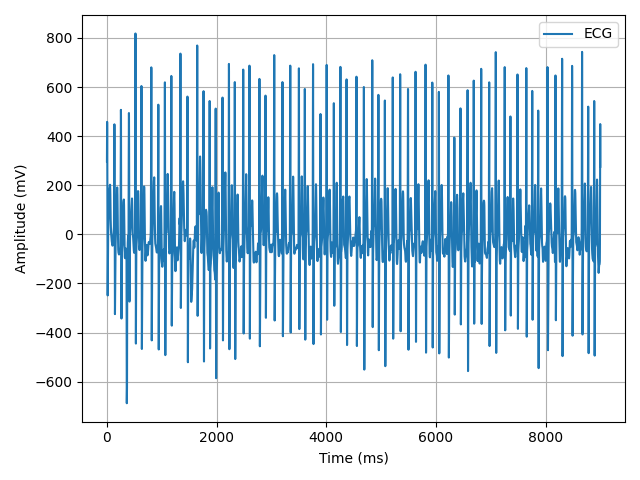
\includegraphics[width=1.0\textwidth, height=0.40\textheight]{Raw_ECG.png}
	\caption{\en Original ECG before preprocessing.}
	\label{original_ECG}
\end{figure}

\begin{figure}[H]
	\centering
	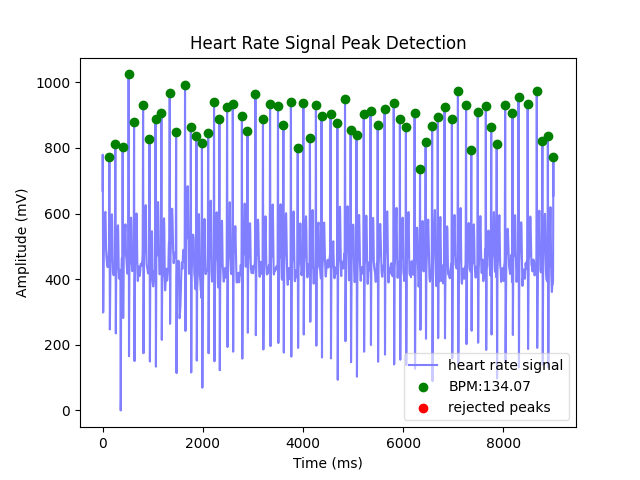
\includegraphics[width=1.0\textwidth, height=0.40\textheight]{Scaled_ECG.png}
	\caption{\en Scaled ECG.}
	\label{Scaled_ECG}
\end{figure}

\begin{figure}[H]
	\centering
	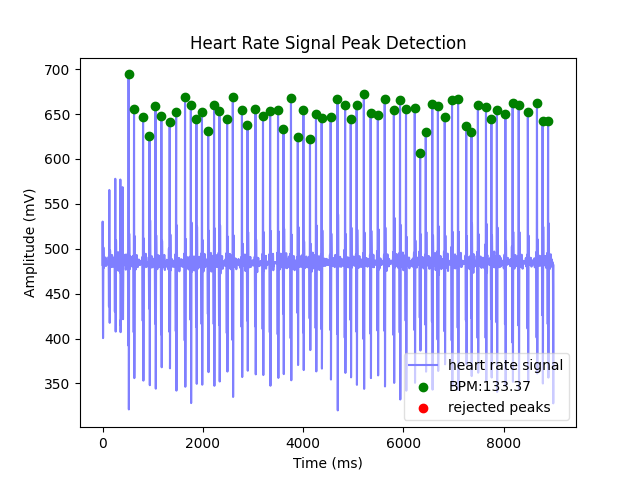
\includegraphics[width=1.0\textwidth, height=0.40\textheight]{Enchanced_ECG.png}
	\caption{\en Enchanced ECG.}
	\label{Enchanced_ECG}
\end{figure}


\section{Processing}

\subsection{R Peak Detection}
To detect R peaks, a moving average is calculated using a window of 1.5 seconds. Regions of interest are marked between two points of intersection (with the moving average) where the signal amplitude is larger than the moving average. R peaks are marked at the maximum of each region of interest. The R peaks are labeled with dots as shown in Figure \hyperref[Enchanced_ECG]{3}.


\subsection{Feature Extraction}
Based on the detected R peaks the following measures are calculated:
\begin{itemize}
	\item Beats per minute  (BPM)
	\item Interbeat interval (IBI)
	\item Standard deviation of RR intervals (SDNN)
	\item Standard deviation of successive differences (SDSD)
	\item Root mean square of successive differences (RMSSD)
	\item Proportion of successive differences above 20ms (pNN20)
	\item Proportion of successive differences above 50ms (pNN50)
	\item Median absolute deviation of RR intervals (MAD)
	\item Standard deviation 1 of Poincaré plot (SD1)
	\item Standard deviation 2 of Poincaré plot (SD2)
	\item Breathing Rate (BR)
\end{itemize}

\section{Classification}
\subsection{Classification on Original Features}
For the classification task several machine learning algorithms have been used. To evaluate their performance cross validation was used on their Accuracy and F1 score. The machine learning algorithms used for the classification task are the Support Vector Machine with radial basis function kernel, the K Nearest Neighbors classifier with 3 nearest neighors, the Naive Bayes classifier, the Random Forest classifier with gini criterion and the Multilayer Perceptron classifier with two hidden layers of sizes 100 and 50 respectively and relu activation function. The results of classification between normal heart rate and atrial fibrillation are shown in Table \hyperref[tab:Normal_Atrial]{2} and the results of classification between atrial fibrillation and other heart rate are shown in Table \hyperref[tab:Atrial_Other]{3}.

\begin{table}[H]
	\centering
	\begin{tabular}{ | c || c || c |}
		
		\hline
		\textbf{Classifier} & \textbf{Accuracy} & \textbf{F1 Score} \\
		
		\hline
		\textbf{Support Vector Machine} & 0.89 & 0.89 \\
		
		\hline
		\textbf{K Nearest Neighbors} & 0.91 & 0.91\\  
		
		\hline
		\textbf{Naive Bayes} & 0.93 & 0.92\\  
		
		\hline
		\textbf{Random Forest} & 0.95 & 0.95\\ 
		
		\hline
		\textbf{Multilayer Perceptron} & 0.93 & 0.92\\ 
		
		\hline
	\end{tabular}
	\caption{Performance of Classification Between Normal or Atrial Fibrillation.}
	\label{tab:Normal_Atrial}
\end{table}

\begin{table}[H]
	\centering
	\begin{tabular}{ | c || c || c |}
		\hline
		\textbf{Classifier} & \textbf{Accuracy} & \textbf{F1 Score} \\
		
		\hline
		\textbf{Support Vector Machine} & 0.80 & 0.81 \\
		
		\hline
		\textbf{K Nearest Neighbors} & 0.81 & 0.82\\  
		
		\hline
		\textbf{Naive Bayes} & 0.81 & 0.80\\  
		
		\hline
		\textbf{Random Forest} & 0.89 & 0.88\\ 
		
		\hline
		\textbf{Multilayer Perceptron} & 0.86 & 0.86\\ 
		
		\hline
	\end{tabular}
	\caption{Performance of Classification Between Atrial Fibrillation or Other.}
	\label{tab:Atrial_Other}
\end{table}


\subsection{Classification on Standardized Features}
To improve the classification performance, the extracted features were transformed with the standardization method. The results of classification between normal heart rate and atrial fibrillation are shown in Table \hyperref[tab:Normal_Atrial_St]{4} and the results of classification between atrial fibrillation and other heart rate are shown in Table \hyperref[tab:Atrial_Other_St]{5}.

\begin{table}[H]
	\centering
	\begin{tabular}{ | c || c || c |}
		
		\hline
		\textbf{Classifier} & \textbf{Accuracy} & \textbf{F1 Score} \\
		
		\hline
		\textbf{Support Vector Machine} & 0.96 & 0.96 \\
		
		\hline
		\textbf{K Nearest Neighbors} & 0.96 & 0.96\\  
		
		\hline
		\textbf{Naive Bayes} & 0.94 & 0.94\\  
		
		\hline
		\textbf{Random Forest} & 0.95 & 0.95\\ 
		
		\hline
		\textbf{Multilayer Perceptron} & 0.94 & 0.94\\ 
		
		\hline
	\end{tabular}
	\caption{Performance of Classification Between Normal or Atrial Fibrillation.}
	\label{tab:Normal_Atrial_St}
\end{table}

\begin{table}[H]
	\centering
	\begin{tabular}{| c || c || c |}
		\hline
		\textbf{Classifier} & \textbf{Accuracy} & \textbf{F1 Score} \\
		
		\hline
		\textbf{Support Vector Machine} & 0.90 & 0.90 \\
		
		\hline
		\textbf{K Nearest Neighbors} & 0.88 & 0.88\\  
		
		\hline
		\textbf{Naive Bayes} & 0.83 & 0.83\\  
		
		\hline
		\textbf{Random Forest} & 0.89 & 0.88\\ 
		
		\hline
		\textbf{Multilayer Perceptron} & 0.87 & 0.87\\ 
		
		\hline
	\end{tabular}
	\caption{Performance of Classification Between Atrial Fibrillation or Other.}
	\label{tab:Atrial_Other_St}
\end{table}


\section{Conclusions}
Based on the experimental results the electrocardiogram contains a lot of useful information with which the electrocardiographs can be correctly classified. The extracted features seem to be powerful for this kind of task and combined with machine learning methods the automated classification of electrocardiographs between the chosen classes has been achieved with good performance. The best results were accomplished with the Support Vector Machines in both classification tasks with Accuracy of 0.96 and F1 score of 0.96 in the first task and Accuracy of 0.90 and F1 score of 0.90 in the second task.


\section{Main Libraries Used in Project}
The program is written in Python 3. For the electrocardiographs preprocessing and processing the \href{https://pypi.org/project/heartpy}{heartpy} library was used. For the machine learning methods the \href{https://scikit-learn.org/}{scikit} library was used. For the plots the \href{https://matplotlib.org/}{matplotlib} library was used.

\section{Notes}
To execute the program adjust the path to the training2017 dataset at line 178 in the project.py file. After that execute python3 project.py in the terminal.

\end{document}